\documentclass[10pt]{article}
\usepackage[margin=0.75in]{geometry}\usepackage[T1]{fontenc}\usepackage{amsmath,amssymb,tikz,url}
\begin{document}\section*{Collector row signs and target information}
\textbf{Offline software result; independent source-fidelity review pending.}

The native collector stores $[A,b,d]$ with $d=-a$ and returns $d/b$ after nuisance elimination. The offline information diagnostic declares $Ax+bk+c=0$. Its corresponding row is therefore $[A,b,-d]$. The adapter changes only that last coefficient.
\begin{center}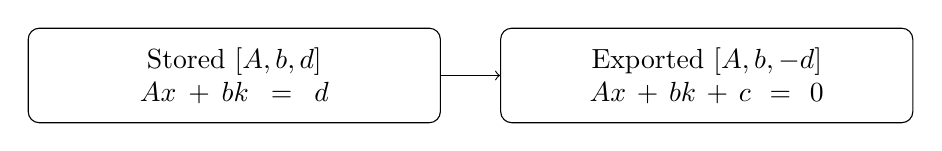
\begin{tikzpicture}[every node/.style={draw,rounded corners,align=center,text width=5cm,minimum height=1.2cm}]
\node (a) at (-3,0) {Stored $[A,b,d]$\\$Ax+bk=d$};
\node (b) at (3,0) {Exported $[A,b,-d]$\\$Ax+bk+c=0$};
\draw[->] (a)--(b);
\end{tikzpicture}\end{center}
\subsection*{A sign error can pass every rank check}
For the stored row $[0,1,5]$ over $\mathbf F_7$, the converted homogeneous row is $[0,1,2]$ and its target is $k=5$. Reading the stored row unchanged as homogeneous gives $k=2$. Both rank triples are $(0,1,1)$ and both systems are consistent with a unique target.

More generally, multiplying the entire constant column by $-1$ preserves rank. The nuisance and nuisance-plus-target matrices are identical; the full matrices differ by an invertible diagonal column transformation. Negation of every unknown gives a bijection between the two homogeneous solution sets. Thus rank, consistency and unique-target booleans alone do not check this sign convention.
\subsection*{Fixed software controls}
All 125 one-row triples over $\mathbf F_5$ and all 343 over $\mathbf F_7$ were enumerated. Complete $(x,k)$ solution sets were checked against a separately written right-hand-side predicate. Six additional fixed systems cover empty, nuisance-only, nonzero target-only, two-row target determination, inconsistent constant-only and target-zero cases. Eight malformed input cases were rejected.

A fresh isolated CLI linked to the existing Rust information diagnostic checked both encodings for each of the 474 systems: 948 outputs. All three ranks, consistency and target-determination outputs matched the explicit solution-set checks. Source inventories were unchanged. These are same-producer cross-implementation checks, not an independent review or a timing comparison. Raw per-case records and the native input/output stream accompany this report.
\subsection*{Source interpretation and boundaries}
The source constructs $D=\tau(aG+bH)$ and verifies $D+\sum P_i=0$ before insertion. To interpret nuisance columns as scalar values, this packet explicitly assumes an additive transfer and a valid homomorphism to $\mathbf F_r$ sending $\tau(G)$ to $1$ and $\tau(H)$ to $k$. Then the verified relation gives $Ax+bk+a=0$. Under that hypothesis, zero-ordinate 2-torsion terms map to zero for odd $r$. The existence and normalization of this homomorphism, arbitrary point labels, and real retained relation streams are not certified here.

The adapter validates canonical integer residues modulo an integer at least2; admission is not a primality certificate. Rank arguments require a field. The enumerated fields here are exactly 5 and 7. No runtime collector code, scientific workload, cohort result or cost ratio changed.
\subsection*{Custody and next integration step}
Sources: \texttt{native\_solver.rs} lines 471--515, 1058--1119, 1311--1359; existing \texttt{rank-information/src/lib.rs}; Sage's primary matrix reference, \url{https://doc.sagemath.org/html/en/reference/matrices/sage/matrix/matrix2.html}, for right-hand-side equation conventions (Sage itself was not executed).

\texttt{source-slices.json} binds exact source bytes. \texttt{status.json}, per-field rows, fixed controls, native receipts and input hashes are retained. The editable diagram is \texttt{flow.svg}. Next: independent source review, then bind an actual retained stream and its subgroup projection before prospective collector-policy measurement.
\end{document}
